%----------------------------------------------------------------------------------------
%	SLIDE 1.
%----------------------------------------------------------------------------------------
\begin{frame}
\frametitle{Projects and goals}

\begin{itemize}
	\item<1-> \textbf{GADGET-2}
	\begin{itemize}
		\item<1-> Simulate an isolated, rotating galaxy with and without dark matter
		\item<1-> Compare their rotation curves to each other and to reality
	\end{itemize}
\end{itemize}
\begin{figure}
	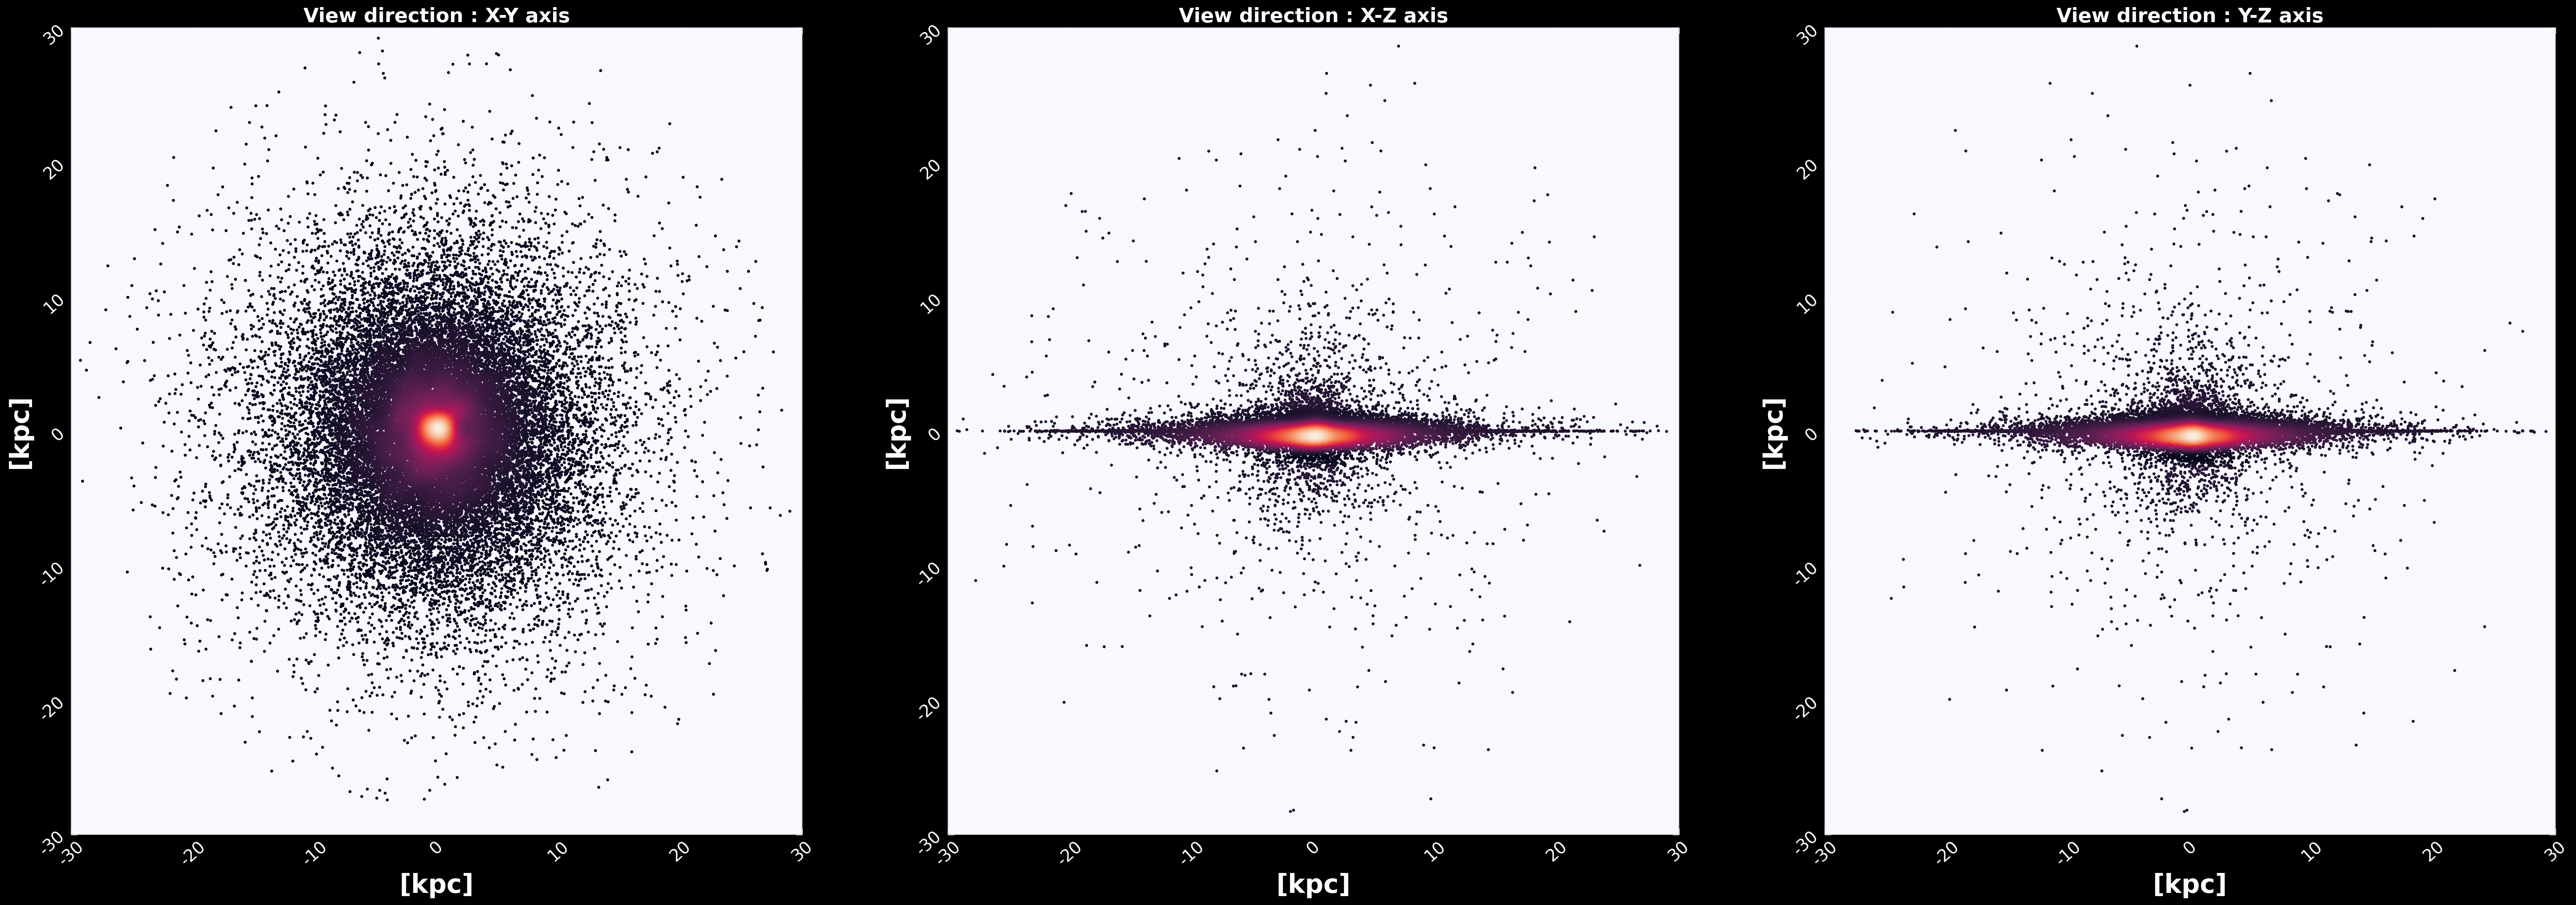
\includegraphics[width=0.9\textwidth]{./images/galaxy_init.png}
	\captionof{figure}{Initial conditions of my rotating galaxy simulation, where only those particles are shown, which are part of the bulge, gas or disk parts of the galaxy. The particles of the halo are hidden here.}
\end{figure}

\end{frame}